\paragraph{Цель работы}
Научиться использовать библиотеку элементов графического интерфейса Qt.

\paragraph{Задание 1}
пользуясь примером в каталоге lab08/02, создайте приложение с графическим интерфейсом, аналогичным представленному сверху
используйте классы QLabel, QSpinBox, QSlider, QPlainTextEdit.

\lstinputlisting[language=C++]{../../src/QT/1/1/mainwindow.h}
\lstinputlisting[language=C++]{../../src/QT/1/1/mainwindow.cpp}

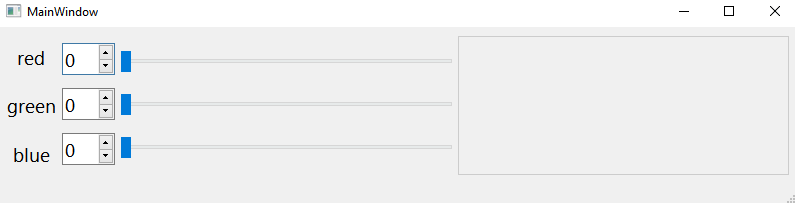
\includegraphics[width=0.6\textwidth]{scr1.PNG}

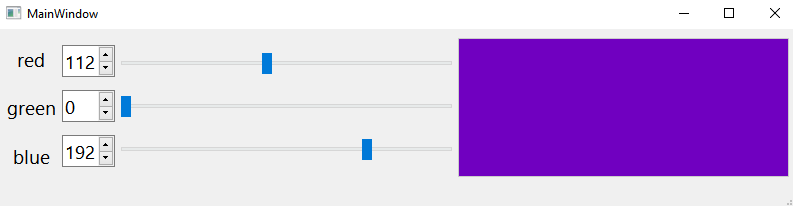
\includegraphics[width=0.6\textwidth]{scr2.PNG}

\paragraph{Задание 2}
Создать простейший обозреватель текстовых файлов.

\lstinputlisting[language=C++]{../../src/QT/1/file_explorer/mainwindow.h}
\lstinputlisting[language=C++]{../../src/QT/1/file_explorer/mainwindow.cpp}

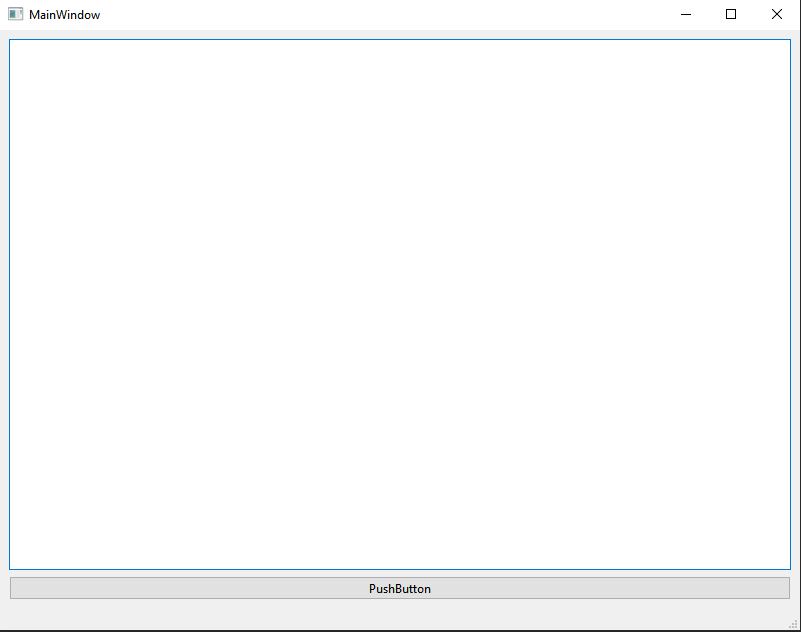
\includegraphics[width=0.6\textwidth]{scr3.PNG}


\includegraphics[width=0.6\textwidth]{scr4.PNG}

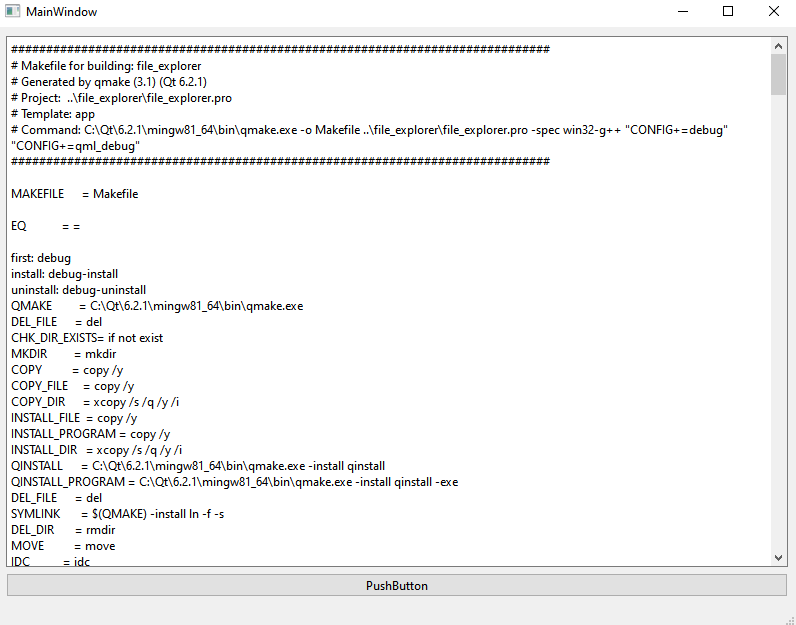
\includegraphics[width=0.6\textwidth]{scr5.PNG}